\section{Sprint 1: base del sistema}
\subsection{Objetivo y alcance}
El Sprint 1 estableció la base técnica y funcional: cuentas y roles, reglas y umbrales, catálogo de carreras y asignaturas, entrada central mediante Gateway, registro de expedientes con PDF y publicación de solicitudes en RabbitMQ. La planificación original identificó las historias como US-01 a US-06; aquí se presentan con la nomenclatura HU-01 a HU-06.

\subsection{Sprint Backlog}
\begin{tabularx}{\textwidth}{|c|X|c|}\hline
\rowcolor{grisTarjeta}\textbf{Historia} & \textbf{Alcance} & \textbf{SP}\\\hline
HU-01 & Cuentas, autenticación y roles & 5\\\hline
HU-02 & Reglas y umbrales & 5\\\hline
HU-03 & Carreras, mallas y asignaturas & 5\\\hline
HU-04 & API Gateway (habilitadora) & 5\\\hline
HU-05 & Registrar expedientes y PDF & 8\\\hline
HU-06 & Publicar solicitudes en RabbitMQ (habilitadora) & 5\\\hline
\multicolumn{2}{|r|}{Total} & 33\\\hline
\end{tabularx}
\captionof{table}{Sprint Backlog del Sprint 1}

\subsection{Historias, criterios y tareas}
\subsubsection{HU-01: Cuentas y roles}
\historia{HU-01}{Administrador del sistema}{Gestión de cuentas y roles}{Alta}{Media}{5 SP}{Sprint 1}{Jair León; Paul Acurio; Alex Jonathan Chisag; Rolando Sebastián Miranda}{Como administrador, quiero crear y gestionar cuentas con roles, para que cada persona acceda solo a las funciones autorizadas.}{\item Dado un registro válido, cuando se crea una cuenta, entonces se asigna el rol solicitado y la contraseña se guarda como hash.\item Dado un usuario activo, cuando sus credenciales son correctas, entonces obtiene una sesión con su rol.\item Dado un rol sin permiso o un correo duplicado, cuando intenta gestionar cuentas, entonces la operación se rechaza.}{Historia denominada US-01 en la fuente.}{M-01 (Inicio de sesión institucional)}
\casosdeuso{HU-01}{Administrador}{{Iniciar sesión},{Crear cuenta con rol},{Validar correo único},{Activar o desactivar\\cuenta}}{1,2,4}{\incluye{2}{3}}{El administrador inicia sesión y gestiona las cuentas; al crear una cuenta siempre se valida que el correo no esté repetido.}
\par\needspace{8\baselineskip}\noindent\textbf{\textit{Desglose de tareas -- HU-01}}\par
La historia se divide en 7 tareas que suman 20,3 horas.\par\medskip
\tarea{S1-J01}{HU-01}{Definición de contratos REST y migraciones iniciales en DB A}{D}{2,9 h}{Día 1 del Sprint 1}{Día 1 del Sprint 1}{Jair Alexander León Tusa}{Definir los contratos REST de usuarios, reglas y catálogo académico, y generar las migraciones iniciales con Entity Framework Core para las tablas USUARIO y ROL en SQL Server DB A.}
\tarea{S1-S01}{HU-01}{Configuración de contenedores Docker Compose para bases de datos y servicios}{O}{2,9 h}{Día 1 del Sprint 1}{Día 1 del Sprint 1}{Rolando Sebastián Miranda Baño}{Configurar el archivo docker-compose.yml para levantar las instancias aisladas de SQL Server (DB A, DB B, DB C), RabbitMQ y los microservicios .NET Core 8 verificando conectividad de red.}
\tarea{S1-J02}{HU-01}{Implementación de alta de usuarios, hash BCrypt y gestión de estado/rol}{D}{2,9 h}{Día 2 del Sprint 1}{Día 2 del Sprint 1}{Jair Alexander León Tusa}{Implementar en el Microservicio A los endpoints de creación y actualización de cuentas, aplicando cifrado BCrypt a las contraseñas, validación de correo institucional único y control de estado activo/inactivo.}
\tarea{S1-S02}{HU-01}{Implementación de autenticación JWT con claims de rol y expiración}{D}{2,9 h}{Día 2 del Sprint 1}{Día 2 del Sprint 1}{Rolando Sebastián Miranda Baño}{Implementar el servicio emisor de tokens JWT firmados en el Microservicio A, inyectando los claims de identidad y rol ( ADMINISTRADOR, DOCENTE, OPERADOR ) y rechazando cuentas inactivas o credenciales inválidas.}
\tarea{S1-A02}{HU-01}{Construcción de vista de inicio de sesión y manejo de sesión en React}{D}{2,9 h}{Día 2 del Sprint 1}{Día 2 del Sprint 1}{Alex Jonathan Chisag Punina}{Desarrollar en React 18 + TypeScript la pantalla de acceso institucional, el almacenamiento seguro del token JWT en sesión y el bloqueo visual de rutas restringidas con pantalla de acceso denegado.}
\tarea{S1-P02}{HU-01}{Verificación de matriz de permisos RBAC por rol}{M}{2,9 h}{Día 2 del Sprint 1}{Día 2 del Sprint 1}{Paul Medardo Acurio López}{Revisar y ejecutar las pruebas de autorización para los roles Administrador, Docente y Operador sobre los endpoints de cuentas, documentando la matriz de accesos válidos ( 200/201) y denegados (401/403).}
\tarea{S1-S03}{HU-01}{Pruebas unitarias de autenticación RBAC en xUnit y esquema DB B}{C}{2,9 h}{Día 3 del Sprint 1}{Día 3 del Sprint 1}{Rolando Sebastián Miranda Baño}{Codificar pruebas unitarias en xUnit + Moq para validar el bloqueo RBAC y emisión JWT (1,7 h) y generar las migraciones iniciales de expedientes en SQL Server DB B (1,2 h).}
\par\needspace{14\baselineskip}\noindent\textbf{\textit{Mockup de HU-01}}\par
\begin{figure}[H]\centering\fbox{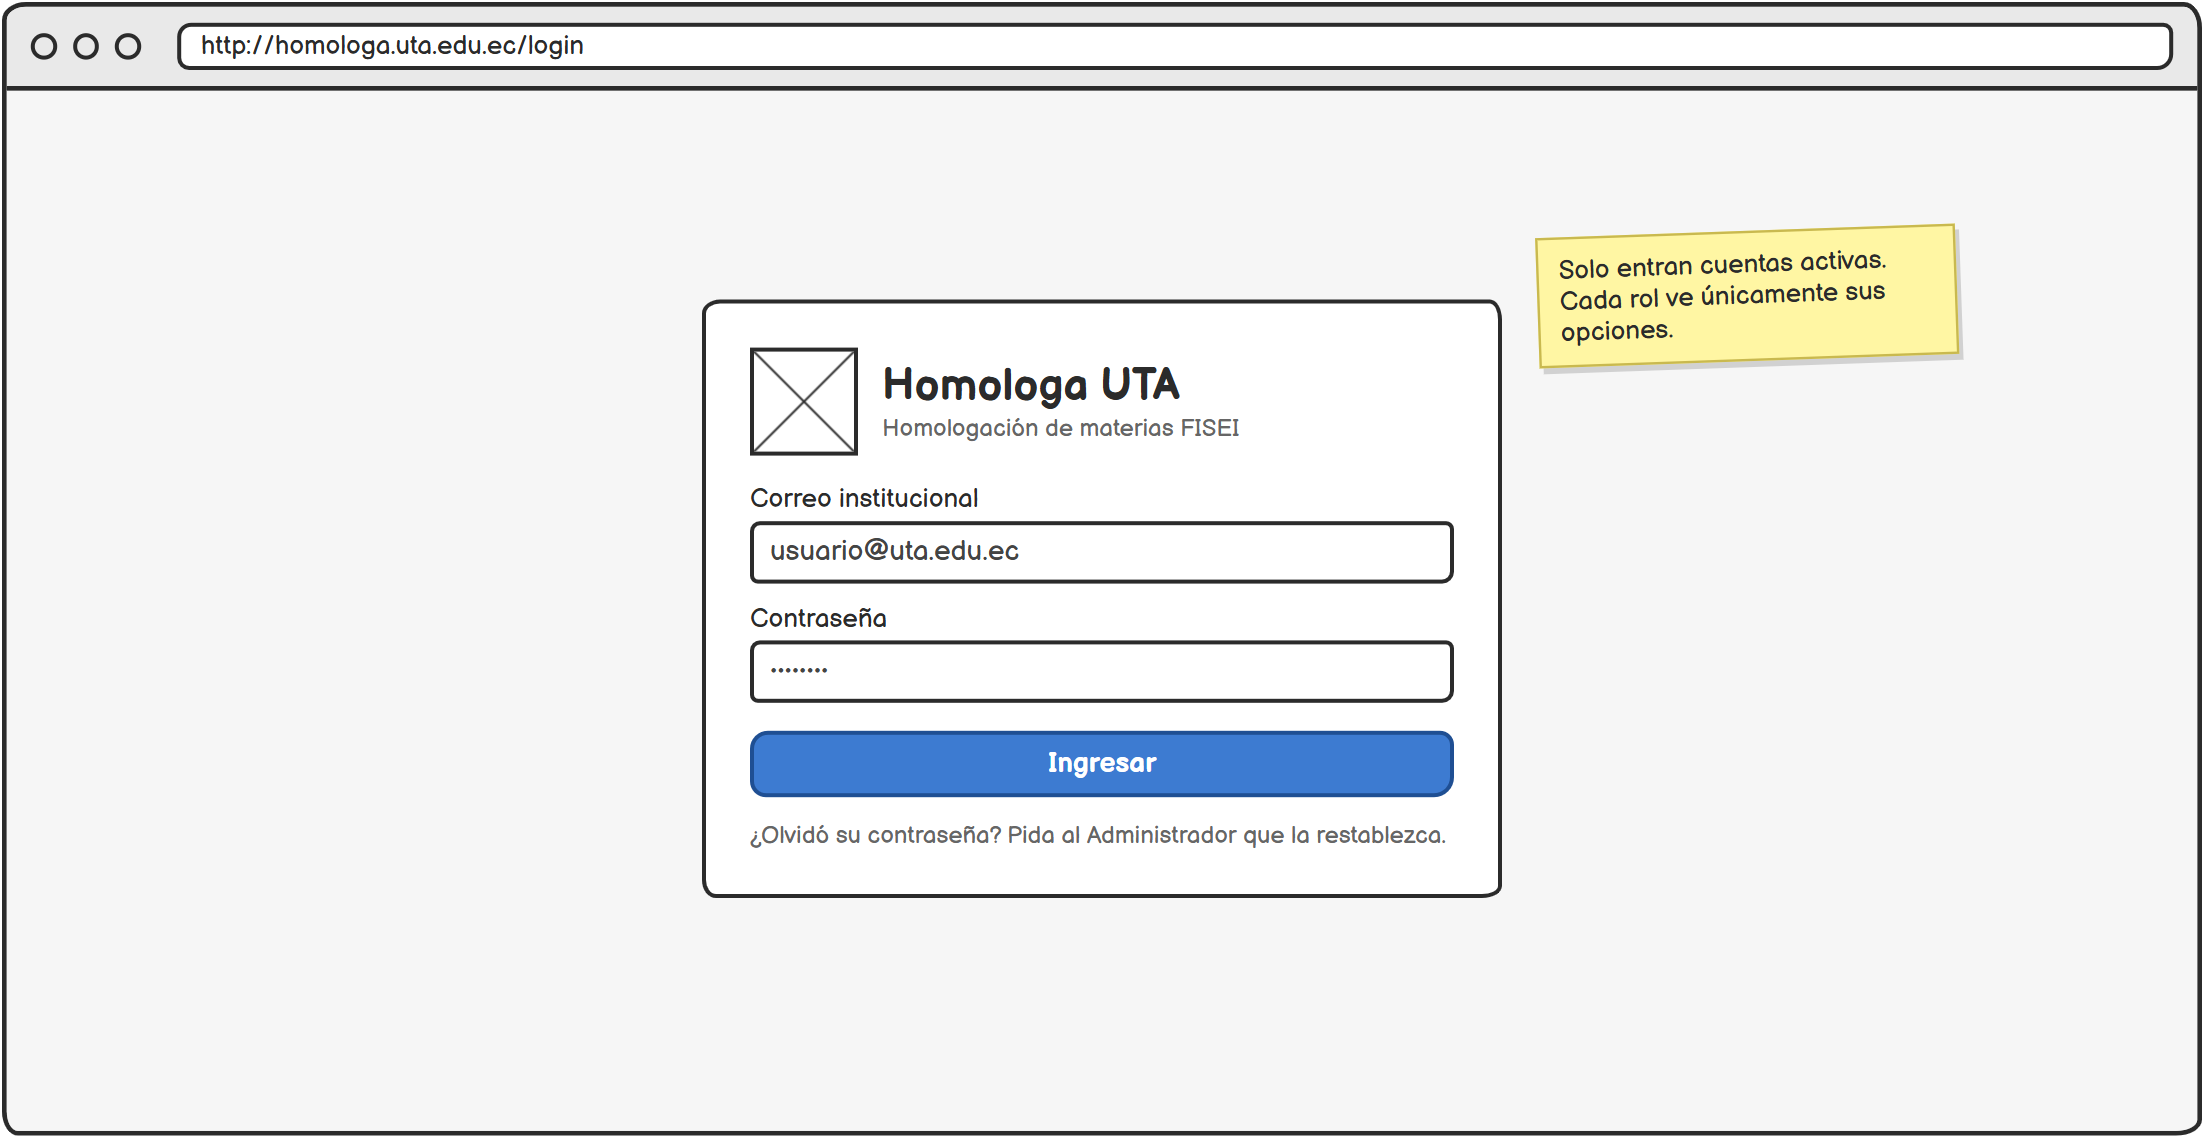
\includegraphics[width=0.93\textwidth]{mockups/m01.png}}
\caption{Mockup M-01 -- Inicio de sesión institucional}
\end{figure}
\par\needspace{6\baselineskip}\noindent\textbf{\textit{Pruebas de aceptación -- HU-01}}\par
\begin{longtable}{|p{1.4cm}|p{3.7cm}|p{4.6cm}|p{5.1cm}|}
\hline\rowcolor{grisTarjeta}\textbf{N.º} & \textbf{Prueba} & \textbf{Entrada} & \textbf{Resultado esperado}\\\hline
\endhead
PA-01.1 & Lista de cuentas con su rol y estado & El administrador abre Usuarios y roles. & Cuentas con rol, estado y acciones\\\hline
PA-01.2 & Crear una cuenta con datos que no coinciden & El administrador intenta crear una cuenta escribiendo dos contraseñas distintas. & ``Las contraseñas no coinciden''; no se crea\\\hline
PA-01.3 & Un rol sin permiso entra a Usuarios y roles & El operador escribe a mano la dirección de Usuarios y roles. & ``No tiene acceso a esta sección''\\\hline
\caption{Pruebas de aceptación de la HU-01}
\end{longtable}

\subsubsection{HU-02: Reglas y umbrales}
\historia{HU-02}{Administrador del sistema}{Reglas y umbrales configurables}{Alta}{Media}{5 SP}{Sprint 1}{Jair León; Paul Acurio; Alex Jonathan Chisag; Rolando Sebastián Miranda}{Como administrador, quiero configurar reglas y umbrales, para aplicar de forma consistente los criterios acordados.}{\item Dado un umbral válido, cuando se guarda, entonces queda asociado a su trámite, fuente y vigencia.\item Dado un valor fuera del rango permitido, cuando se actualiza, entonces se rechaza sin reemplazar la configuración vigente.\item Dado un usuario sin rol administrador, cuando modifica reglas, entonces se deniega la operación.}{La fuente la denomina US-02.}{M-02 (Configurar el mínimo para homologar)}
\casosdeuso{HU-02}{Administrador}{{Consultar reglas vigentes},{Cambiar el mínimo (80~\%)},{Guardar nueva versión},{Ver historial de versiones}}{1,2,4}{\incluye{2}{3}}{Cada cambio del mínimo se guarda como una nueva versión de la regla; el mínimo no puede bajar de 80~\%.}
\par\needspace{8\baselineskip}\noindent\textbf{\textit{Desglose de tareas -- HU-02}}\par
La historia se divide en 5 tareas que suman 14,5 horas.\par\medskip
\tarea{S1-J03}{HU-02}{Implementación de API REST de consulta y actualización de reglas y umbrales}{D}{2,9 h}{Día 3 del Sprint 1}{Día 3 del Sprint 1}{Jair Alexander León Tusa}{Implementar en el Microservicio A los endpoints REST para consultar y actualizar los umbrales de créditos y de contenidos y las reglas de cada trámite, validando que los valores estén en rango y que solo el Administrador pueda cambiarlos.}
\tarea{S1-A03}{HU-02}{Construcción del formulario web de reglas y parámetros de evaluación}{D}{2,9 h}{Día 3 del Sprint 1}{Día 3 del Sprint 1}{Alex Jonathan Chisag Punina}{Construir en React 18 el formulario de configuración de reglas con selector de ruta de trámite (CAU-P-011 / CAU-P-122), campos para los umbrales de créditos y contenidos, validaciones de rango y estados de guardado/error.}
\tarea{S1-P03}{HU-02}{Pruebas de validación de rangos y permisos en configuración de umbrales}{M}{2,9 h}{Día 3 del Sprint 1}{Día 3 del Sprint 1}{Paul Medardo Acurio López}{Probar la configuración de umbrales con valores válidos, valores fuera de rango (negativos, mayores que 100~\% o umbrales incoherentes entre sí) y peticiones con roles no autorizados, documentando las evidencias positivas y negativas.}
\tarea{S1-S04}{HU-02}{Implementación del servidor gRPC de reglas en Microservicio A}{D}{2,9 h}{Día 4 del Sprint 1}{Día 4 del Sprint 1}{Rolando Sebastián Miranda Baño}{Definir el contrato reglas.proto e implementar el servidor ReglasGrpc en el Microservicio A para exponer con baja latencia los umbrales vigentes hacia el Microservicio C.}
\tarea{S1-A08}{HU-02}{Integración de acceso, umbrales y catálogo con Microservicio A vía Gateway}{C}{2,9 h}{Día 8 del Sprint 1}{Día 8 del Sprint 1}{Alex Jonathan Chisag Punina}{Conectar los formularios de inicio de sesión, reglas y catálogo académico con los servicios reales del Microservicio A a través del API Gateway, retirando los mocks iniciales.}
\par\needspace{14\baselineskip}\noindent\textbf{\textit{Mockup de HU-02}}\par
\begin{figure}[H]\centering\fbox{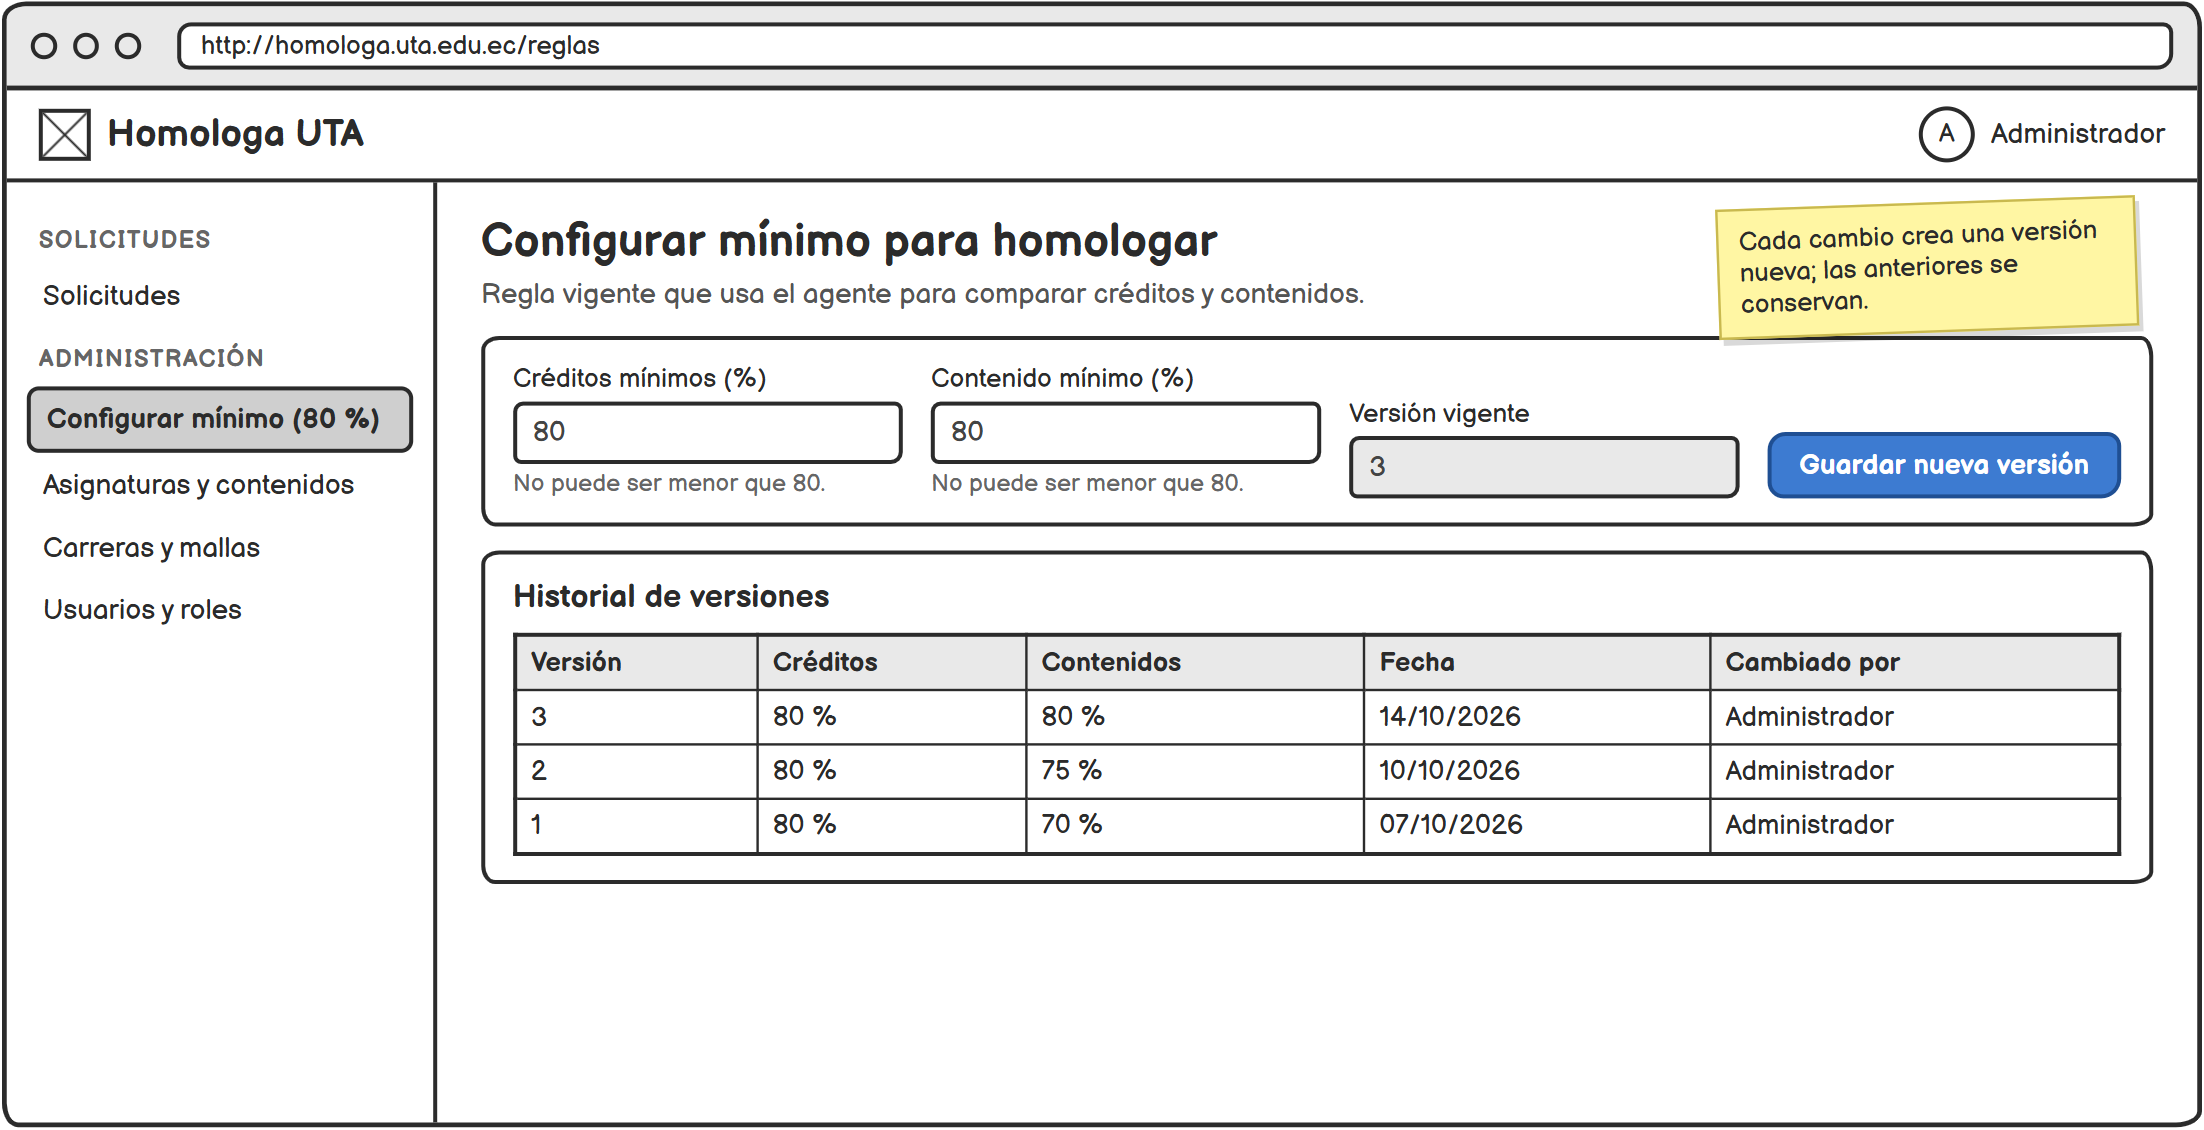
\includegraphics[width=0.93\textwidth]{mockups/m02.png}}
\caption{Mockup M-02 -- Configurar el mínimo para homologar}
\end{figure}
\par\needspace{6\baselineskip}\noindent\textbf{\textit{Pruebas de aceptación -- HU-02}}\par
\begin{longtable}{|p{1.4cm}|p{3.7cm}|p{4.6cm}|p{5.1cm}|}
\hline\rowcolor{grisTarjeta}\textbf{N.º} & \textbf{Prueba} & \textbf{Entrada} & \textbf{Resultado esperado}\\\hline
\endhead
PA-02.1 & Reglas vigentes y catálogo normativo & El administrador abre Configurar mínimo (80~\%). & Mínimo 80~\% y catálogo RN\\\hline
PA-02.2 & Intentar bajar el mínimo de 80~/~\% & El administrador escribe 70 en Contenido mínimo y guarda. & Rechazado con mensaje claro\\\hline
\caption{Pruebas de aceptación de la HU-02}
\end{longtable}

\subsubsection{HU-03: Carreras, mallas y asignaturas}
\historia{HU-03}{Administrador y operador}{Carreras, mallas y asignaturas}{Alta}{Media}{5 SP}{Sprint 1}{Jair León; Alex Jonathan Chisag; Paul Acurio}{Como administrador, quiero gestionar carreras, mallas y asignaturas, para que el operador pueda seleccionar las materias del caso.}{\item Dado un plan académico, cuando se consulta, entonces se identifican carrera, versión, asignatura, créditos, horas y unidades disponibles.\item Dado un código duplicado, cuando se carga, entonces el sistema lo rechaza.}{La fuente la denomina US-03.}{M-03 (Asignaturas de la malla)}
\casosdeuso{HU-03}{Administrador}{{Consultar carreras y mallas},{Registrar asignaturas\\por nivel},{Validar créditos y nivel},{Consultar contenidos\\de la asignatura}}{1,2,4}{\incluye{2}{3}}{Al registrar una asignatura siempre se validan sus créditos y su nivel dentro de la malla.}
\par\needspace{8\baselineskip}\noindent\textbf{\textit{Desglose de tareas -- HU-03}}\par
La historia se divide en 5 tareas que suman 14,5 horas.\par\medskip
\tarea{S1-J04}{HU-03}{Implementación de CRUD de carreras y versiones de mallas curriculares}{D}{2,9 h}{Día 4 del Sprint 1}{Día 4 del Sprint 1}{Jair Alexander León Tusa}{Implementar en el Microservicio A los controladores y servicios CRUD para las entidades CARRERA y MALLA, validando códigos únicos y relaciones en SQL Server DB A.}
\tarea{S1-A04}{HU-03}{Construcción de listado y formularios web de carreras y mallas}{D}{2,9 h}{Día 4 del Sprint 1}{Día 4 del Sprint 1}{Alex Jonathan Chisag Punina}{Desarrollar en React 18 las vistas de consulta y registro de carreras (Software, TI, Industrial, Robótica, Telecomunicaciones) y versiones de mallas curriculares.}
\tarea{S1-J05}{HU-03}{Implementación de CRUD de asignaturas, unidades e importación de 43 planes}{D}{2,9 h}{Día 5 del Sprint 1}{Día 5 del Sprint 1}{Jair Alexander León Tusa}{Implementar el CRUD de ASIGNATURA y UNIDAD\_TEMATICA y el cargador masivo del catálogo estructurado (43 planes analíticos de Software), validando créditos, horas por unidad y rechazo de duplicados.}
\tarea{S1-A05}{HU-03}{Construcción de interfaz de edición de asignaturas y carga estructurada}{D}{2,9 h}{Día 5 del Sprint 1}{Día 5 del Sprint 1}{Alex Jonathan Chisag Punina}{Completar en React la interfaz de gestión de asignaturas, unidades temáticas y el componente de importación del catálogo estructurado con resumen visual de validación y errores.}
\tarea{S1-P05}{HU-03}{Validación funcional de carga del catálogo, duplicados, créditos y horas}{M}{2,9 h}{Día 5 del Sprint 1}{Día 5 del Sprint 1}{Paul Medardo Acurio López}{Ejecutar pruebas de importación de los 43 planes analíticos de Software, verificando rechazo de códigos duplicados, equivalencia de 48 h/crédito UTA y marcado de planes incompletos.}
\par\needspace{14\baselineskip}\noindent\textbf{\textit{Mockup de HU-03}}\par
\begin{figure}[H]\centering\fbox{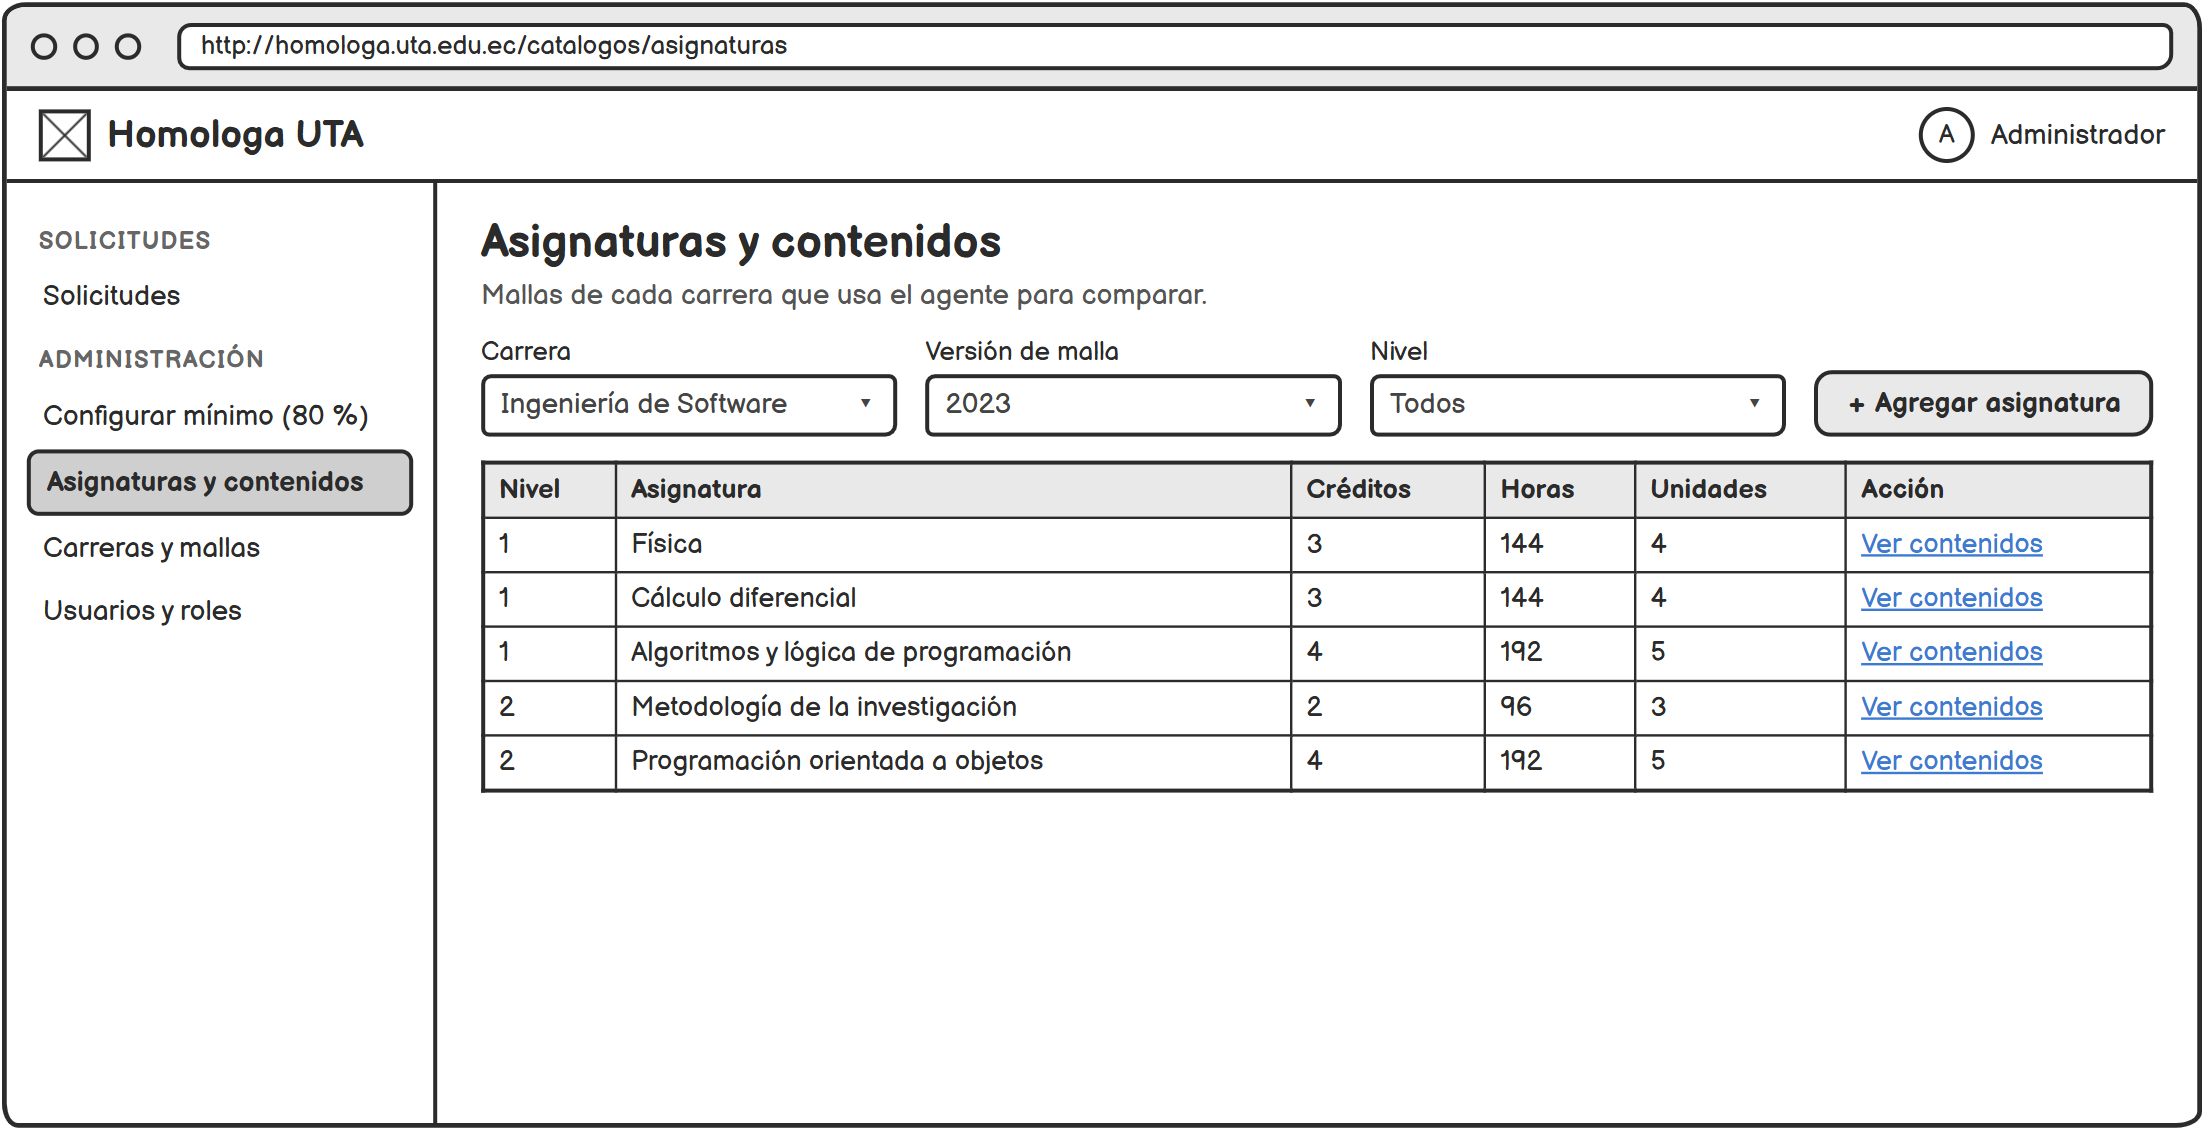
\includegraphics[width=0.93\textwidth]{mockups/m03.png}}
\caption{Mockup M-03 -- Asignaturas de la malla}
\end{figure}
\par\needspace{6\baselineskip}\noindent\textbf{\textit{Pruebas de aceptación -- HU-03}}\par
\begin{longtable}{|p{1.4cm}|p{3.7cm}|p{4.6cm}|p{5.1cm}|}
\hline\rowcolor{grisTarjeta}\textbf{N.º} & \textbf{Prueba} & \textbf{Entrada} & \textbf{Resultado esperado}\\\hline
\endhead
PA-03.1 & Carreras y versiones de malla & El administrador abre Carreras y mallas. & Listado de carreras y versiones\\\hline
PA-03.2 & Asignaturas con créditos, horas y unidades & El administrador abre Asignaturas y contenidos. & Créditos, horas y unidades\\\hline
\caption{Pruebas de aceptación de la HU-03}
\end{longtable}

\subsubsection{HU-04: API Gateway}
\historia{HU-04}{Responsable de arquitectura}{Entrada central con permisos}{Alta}{Media}{5 SP}{Sprint 1}{Jair León; Alex Jonathan Chisag; Rolando Sebastián Miranda; Paul Acurio}{Como responsable de arquitectura, quiero centralizar las rutas y validar los permisos, para dirigir cada petición al servicio correspondiente.}{\item Dado un token válido y permisos adecuados, cuando se envía una petición, entonces llega al servicio previsto.\item Dado un token ausente o un rol sin permiso, cuando se accede a una ruta protegida, entonces el Gateway rechaza la petición.}{Historia habilitadora US-04.}{M-04 (Acceso denegado por rol)}
\casosdeuso{HU-04}{Usuario del sistema}{{Entrar por el Gateway},{Validar la sesión},{Comprobar el permiso\\por rol},{Mostrar acceso denegado}}{1}{\incluye{1}{2}\incluye{2}{3}\extiende{4}{3}}{Toda petición entra por el Gateway, que valida la sesión y el rol; si el rol no tiene permiso, se muestra acceso denegado.}
\par\needspace{8\baselineskip}\noindent\textbf{\textit{Desglose de tareas -- HU-04}}\par
La historia se divide en 5 tareas que suman 14,5 horas.\par\medskip
\tarea{S1-A01}{HU-04}{Preparación de proyecto React, cliente REST con interceptores JWT y mocks}{D}{2,9 h}{Día 1 del Sprint 1}{Día 1 del Sprint 1}{Alex Jonathan Chisag Punina}{Inicializar la SPA en React 18 + Vite + TypeScript, configurar el cliente HTTP centralizado apuntando al API Gateway con inyección de cabeceras Authorization: Bearer y preparar mocks para desarrollo paralelo.}
\tarea{S1-J06}{HU-04}{Configuración de enrutamiento Ocelot, validación JWT y políticas RBAC}{D}{2,9 h}{Día 6 del Sprint 1}{Día 6 del Sprint 1}{Jair Alexander León Tusa}{Configurar las rutas del API Gateway hacia los Microservicios A, B y C, activando la validación de firma de tokens JWT y las restricciones de acceso por rol en el borde.}
\tarea{S1-S07}{HU-04}{Pruebas de integración del API Gateway y conectividad del bus RabbitMQ}{C}{2,9 h}{Día 7 del Sprint 1}{Día 7 del Sprint 1}{Rolando Sebastián Miranda Baño}{Ejecutar pruebas automatizadas de acceso a través del API Gateway y verificar la conectividad del bus de eventos con dependencias aisladas y manejo de errores controlados.}
\tarea{S1-P08}{HU-04}{Auditoría de rutas del Gateway y respuestas HTTP 401, 403 y 404}{M}{2,9 h}{Día 8 del Sprint 1}{Día 8 del Sprint 1}{Paul Medardo Acurio López}{Probar exhaustivamente todas las rutas expuestas en el API Gateway verificando los estados HTTP 401, 403 y 404 según el rol autenticado y la disponibilidad del recurso.}
\tarea{S1-J10}{HU-04}{Corrección de hallazgos de integración y pruebas de humo del backend}{C}{2,9 h}{Día 10 del Sprint 1}{Día 10 del Sprint 1}{Jair Alexander León Tusa}{Corregir hallazgos derivados de la integración entre el API Gateway y los microservicios, ejecutar revisión técnica de código y correr pruebas de humo del Sprint 1.}
\par\needspace{14\baselineskip}\noindent\textbf{\textit{Mockup de HU-04}}\par
\begin{figure}[H]\centering\fbox{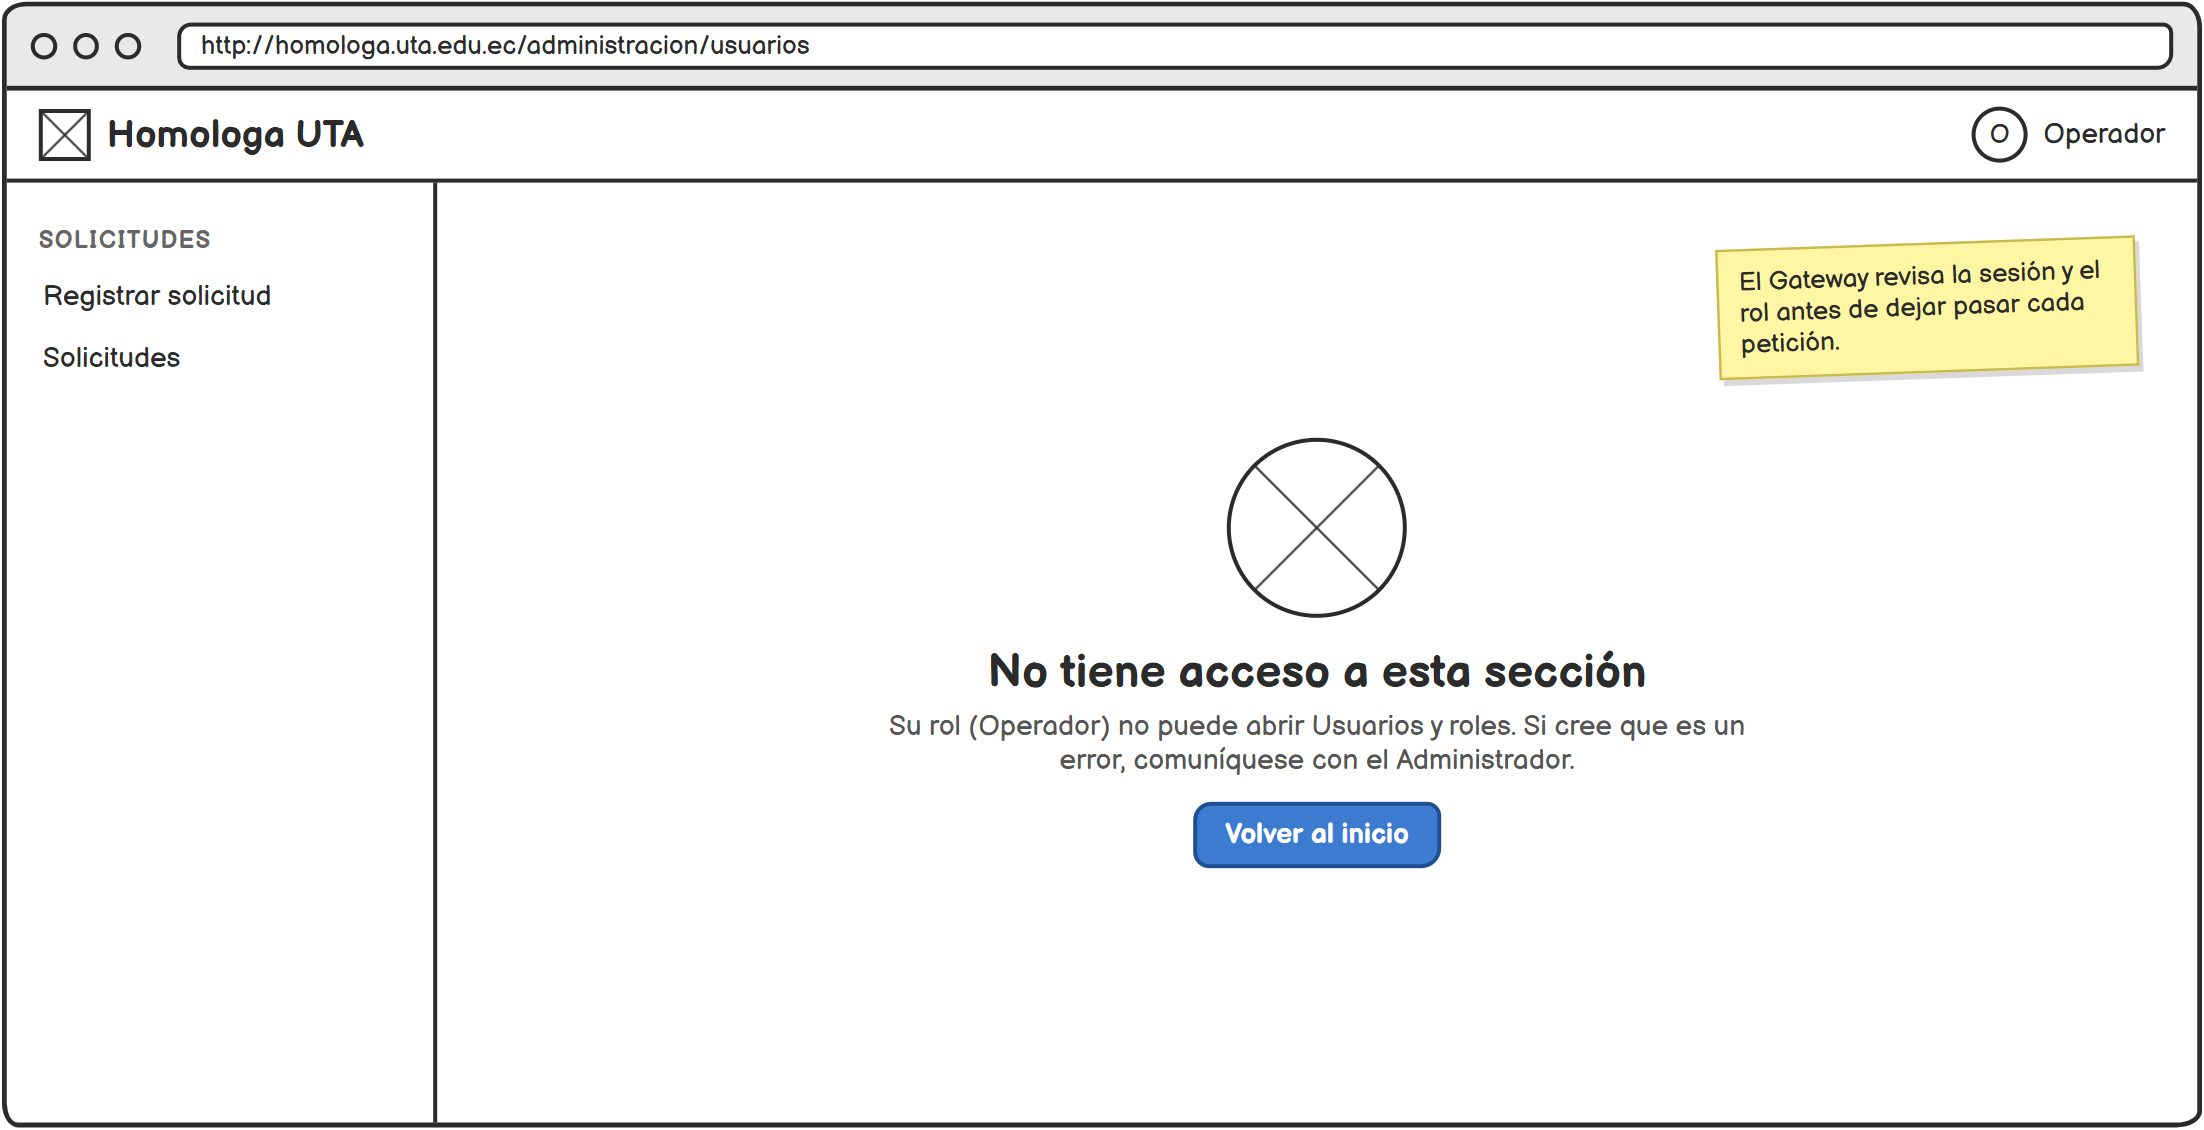
\includegraphics[width=0.93\textwidth]{mockups/m04.png}}
\caption{Mockup M-04 -- Acceso denegado por rol}
\end{figure}
\par\needspace{6\baselineskip}\noindent\textbf{\textit{Pruebas de aceptación -- HU-04}}\par
\begin{longtable}{|p{1.4cm}|p{3.7cm}|p{4.6cm}|p{5.1cm}|}
\hline\rowcolor{grisTarjeta}\textbf{N.º} & \textbf{Prueba} & \textbf{Entrada} & \textbf{Resultado esperado}\\\hline
\endhead
PA-04.1 & Petición sin iniciar sesión & Se pide la lista de usuarios al Gateway sin enviar el JWT. & 401 en el Gateway\\\hline
PA-04.2 & Un docente pide un recurso de administrador & Con la sesión del docente Carlos Paredes se pide la lista de usuarios. & 403 en el Gateway\\\hline
\caption{Pruebas de aceptación de la HU-04}
\end{longtable}

\subsubsection{HU-05: Expedientes y PDF}
\historia{HU-05}{Operador académico}{Registro de expedientes y documentos PDF}{Alta}{Media}{8 SP}{Sprint 1}{Rolando Sebastián Miranda; Alex Jonathan Chisag; Paul Acurio}{Como operador, quiero registrar expedientes internos o externos y adjuntar documentos PDF, para iniciar una solicitud de homologación.}{\item Dado un registro válido, cuando se envía, entonces se genera un identificador y se conserva su tipo de trámite.\item Dado un PDF inválido o información obligatoria ausente, cuando se carga, entonces se informa el error y no se acepta el expediente.}{Historia denominada US-05.}{M-05 (Registrar solicitud con sus PDF)}
\casosdeuso{HU-05}{Operador académico}{{Registrar expediente},{Adjuntar los PDF},{Validar formato y tamaño},{Consultar expedientes}}{1,2,4}{\incluye{2}{3}}{El operador registra el expediente y adjunta los PDF; cada archivo se valida antes de guardarse.}
\par\needspace{8\baselineskip}\noindent\textbf{\textit{Desglose de tareas -- HU-05}}\par
La historia se divide en 8 tareas que suman 23,2 horas.\par\medskip
\tarea{S1-S05}{HU-05}{Implementación de alta de solicitud interna/externa y validación de PDF en B}{D}{2,9 h}{Día 5 del Sprint 1}{Día 5 del Sprint 1}{Rolando Sebastián Miranda Baño}{Implementar en el Microservicio B la lógica de registro de solicitudes internas y externas, selección de materias del catálogo, fecha de aprobación certificada y validación de firma binaria, tamaño y formato de archivos PDF.}
\tarea{S1-S06}{HU-05}{Almacenamiento seguro de PDF y persistencia de metadatos en DB B}{D}{2,9 h}{Día 6 del Sprint 1}{Día 6 del Sprint 1}{Rolando Sebastián Miranda Baño}{Completar el guardado físico seguro de los archivos PDF y su asociación con la tabla EXPEDIENTE\_DOC en SQL Server DB B, habilitando el endpoint de consulta de metadatos y estado de recepción.}
\tarea{S1-A06}{HU-05}{Construcción del formulario web de nueva solicitud y carga de documentos PDF}{D}{2,9 h}{Día 6 del Sprint 1}{Día 6 del Sprint 1}{Alex Jonathan Chisag Punina}{Desarrollar en React 18 el formulario de registro de solicitudes (Interna / Externa), selector de institución de origen, carrera receptora, materias del catálogo y zona de carga de archivos PDF con validación local.}
\tarea{S1-P06}{HU-05}{Pruebas funcionales de alta de expedientes internos y externos}{M}{2,9 h}{Día 6 del Sprint 1}{Día 6 del Sprint 1}{Paul Medardo Acurio López}{Probar el registro de expedientes internos y externos verificando asignaturas seleccionadas, diferenciación de ruta normativa (CAU-P-011 / CAU-P-122) y rechazo ante ausencia de campos obligatorios.}
\tarea{S1-A07}{HU-05}{Integración del formulario de solicitud y carga multipart con Microservicio B}{D}{2,9 h}{Día 7 del Sprint 1}{Día 7 del Sprint 1}{Alex Jonathan Chisag Punina}{Conectar el formulario de registro y subida de archivos PDF con el endpoint real del Microservicio B a través del Gateway, mostrando en pantalla el identificador generado y los mensajes de error devueltos por la API.}
\tarea{S1-P07}{HU-05}{Pruebas de restricciones de archivos PDF (formato, tamaño y permisos)}{M}{2,9 h}{Día 7 del Sprint 1}{Día 7 del Sprint 1}{Paul Medardo Acurio López}{Ejecutar casos de prueba positivos y negativos sobre la carga de documentos: archivos que no son PDF, archivos que superan el tamaño límite, archivos vacíos y accesos con roles no autorizados.}
\tarea{S1-A09}{HU-05}{Verificación integrada de formularios, permisos y fallos de carga en UI}{C}{2,9 h}{Día 9 del Sprint 1}{Día 9 del Sprint 1}{Alex Jonathan Chisag Punina}{Integrar y verificar el comportamiento de los formularios de expedientes internos y externos ante fallos de carga o errores de validación del servidor, registrando los casos de aceptación de la interfaz.}
\tarea{S1-A10}{HU-05}{Revisión de usabilidad, navegación por teclado y preparación de demostración}{M}{2,9 h}{Día 10 del Sprint 1}{Día 10 del Sprint 1}{Alex Jonathan Chisag Punina}{Revisar la accesibilidad por teclado, consistencia de mensajes de validación y preparar la demostración reproducible del flujo del Sprint 1 en la interfaz web.}
\par\needspace{14\baselineskip}\noindent\textbf{\textit{Mockup de HU-05}}\par
\begin{figure}[H]\centering\fbox{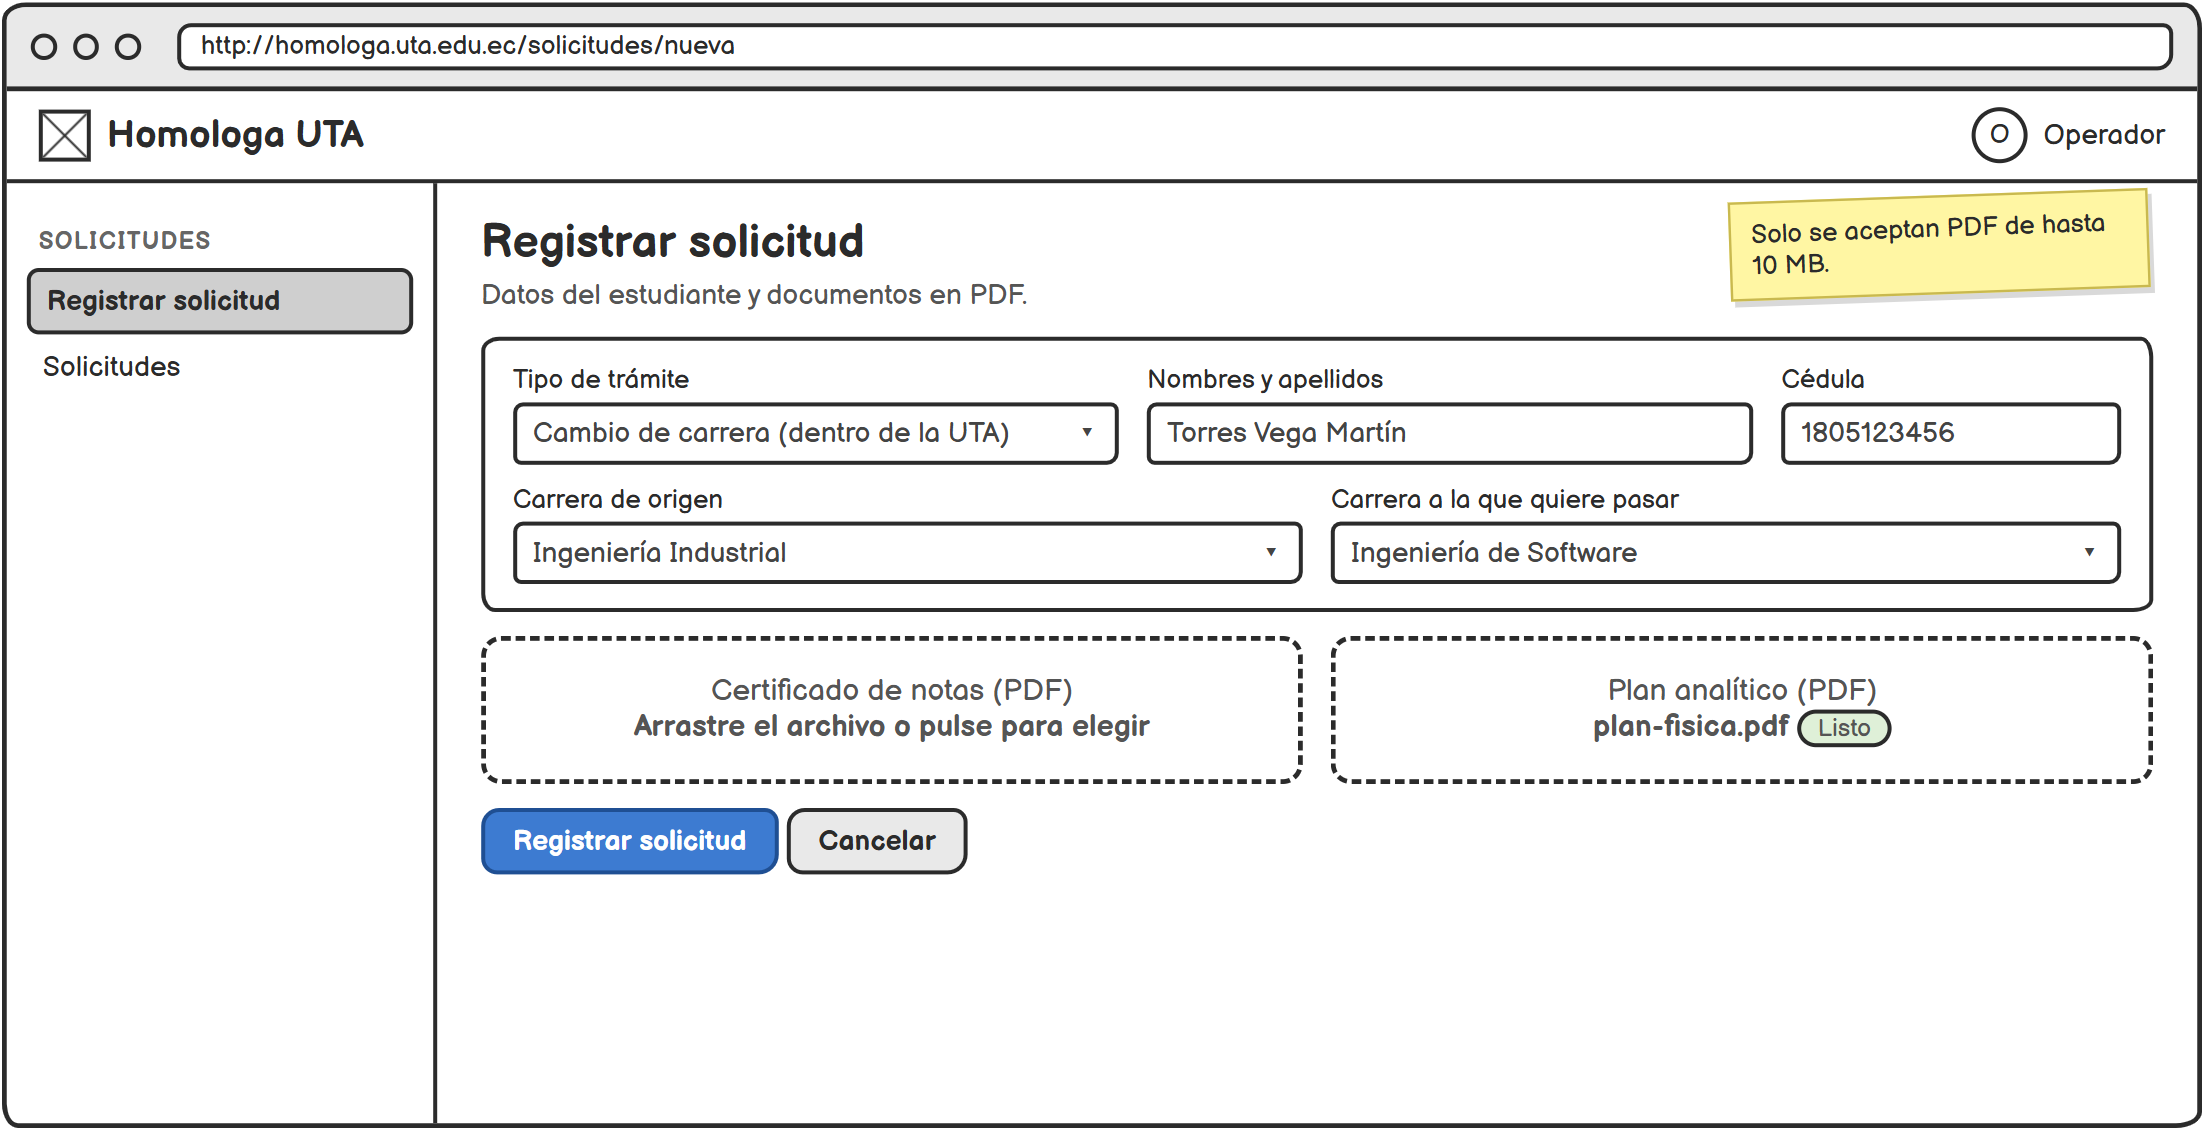
\includegraphics[width=0.93\textwidth]{mockups/m05.png}}
\caption{Mockup M-05 -- Registrar solicitud con sus PDF}
\end{figure}
\par\needspace{6\baselineskip}\noindent\textbf{\textit{Pruebas de aceptación -- HU-05}}\par
\begin{longtable}{|p{1.4cm}|p{3.7cm}|p{4.6cm}|p{5.1cm}|}
\hline\rowcolor{grisTarjeta}\textbf{N.º} & \textbf{Prueba} & \textbf{Entrada} & \textbf{Resultado esperado}\\\hline
\endhead
PA-05.1 & Archivo que no es el certificado & El operador sube un plan analítico suelto (E19) en lugar del certificado. & Rechazado; botón deshabilitado\\\hline
PA-05.2 & Registro de un certificado válido & El operador sube el certificado V05 y lo registra. & Expediente creado y enviado\\\hline
\caption{Pruebas de aceptación de la HU-05}
\end{longtable}

\subsubsection{HU-06: Publicación de solicitudes}
\historia{HU-06}{Responsable de integración}{Publicación de solicitudes en RabbitMQ}{Alta}{Media}{5 SP}{Sprint 1}{Paul Acurio; Rolando Sebastián Miranda}{Como responsable de integración, quiero publicar las solicitudes registradas en RabbitMQ, para que los servicios consumidores puedan procesarlas.}{\item Dado un expediente guardado, cuando se confirma su registro, entonces se publica un evento de solicitud creada.\item Dado que el bus no responde, cuando se intenta publicar, entonces se conserva la posibilidad de reintentar la publicación.}{Historia habilitadora denominada US-06.}{M-06 (Solicitud enviada al análisis)}
\casosdeuso{HU-06}{Operador académico}{{Registrar expediente},{Publicar el aviso\\de solicitud creada},{Recibir el aviso\\una sola vez}}{1}{\incluye{1}{2}\munieco{ana}{(11.2,-3.1)}{Servicio de\\Análisis}\draw (ana-w) -- (c3.east);}{Registrar un expediente incluye publicar el aviso en la cola; el Servicio de Análisis lo recibe una sola vez.}
\par\needspace{8\baselineskip}\noindent\textbf{\textit{Desglose de tareas -- HU-06}}\par
La historia se divide en 10 tareas que suman 29,0 horas.\par\medskip
\tarea{S1-P01}{HU-06}{Definición del contrato SolicitudCreadaEvent e identificador de correlación}{D}{2,9 h}{Día 1 del Sprint 1}{Día 1 del Sprint 1}{Paul Medardo Acurio López}{Definir formalmente la estructura del evento SolicitudCreadaEvent, el identificador de correlación (CorrelationId) y los metadatos mínimos requeridos para el intercambio asíncrono entre B y C.}
\tarea{S1-P04}{HU-06}{Pruebas de publicación en RabbitMQ mediante suscriptor de prueba}{M}{2,9 h}{Día 4 del Sprint 1}{Día 4 del Sprint 1}{Paul Medardo Acurio López}{Implementar y ejecutar un suscriptor de prueba en RabbitMQ para verificar que el mensaje publicado cumpla exactamente el contrato acordado sin activar aún el análisis del Microservicio C.}
\tarea{S1-J07}{HU-06}{Configuración de MassTransit en B y publicación de SolicitudCreadaEvent}{D}{2,9 h}{Día 7 del Sprint 1}{Día 7 del Sprint 1}{Jair Alexander León Tusa}{Configurar el bus MassTransit con RabbitMQ en el Microservicio B e implementar la publicación del evento SolicitudCreadaEvent tras el registro válido de un expediente.}
\tarea{S1-J08}{HU-06}{Vinculación de persistencia con publicación y manejo de reintentos}{D}{2,9 h}{Día 8 del Sprint 1}{Día 8 del Sprint 1}{Jair Alexander León Tusa}{Conectar la persistencia del expediente en DB B con el publicador del bus, configurando políticas de reintento y registro de fallos sin perder la trazabilidad del identificador.}
\tarea{S1-S08}{HU-06}{Configuración de pipeline de Integración Continua (CI) y pruebas automatizadas}{O}{2,9 h}{Día 8 del Sprint 1}{Día 8 del Sprint 1}{Rolando Sebastián Miranda Baño}{Configurar el pipeline de integración continua para compilar automáticamente los microservicios, ejecutar la suite de pruebas xUnit y generar el reporte de resultados en cada cambio.}
\tarea{S1-J09}{HU-06}{Integración de Gateway, expediente y publicador del bus con trazabilidad}{D}{2,9 h}{Día 9 del Sprint 1}{Día 9 del Sprint 1}{Jair Alexander León Tusa}{Integrar el recorrido completo del Sprint 1 desde el API Gateway hasta la persistencia en DB B y la publicación en RabbitMQ, verificando la respuesta HTTP 202 Accepted .}
\tarea{S1-P09}{HU-06}{Verificación de correlación del evento y recuperación ante fallos del bus}{M}{2,9 h}{Día 9 del Sprint 1}{Día 9 del Sprint 1}{Paul Medardo Acurio López}{Ejecutar pruebas de fallo y recuperación desconectando temporalmente RabbitMQ para comprobar que el publicador reintenta el envío conservando el identificador de correlación.}
\tarea{S1-S09}{HU-06}{Ejecución de pruebas integradas de reglas, expedientes, PDF y evento}{C}{2,9 h}{Día 9 del Sprint 1}{Día 9 del Sprint 1}{Rolando Sebastián Miranda Baño}{Ejecutar pruebas integradas de extremo a extremo sobre el flujo de recepción de solicitudes, carga de PDF y publicación del evento en el bus, corrigiendo los defectos detectados.}
\tarea{S1-P10}{HU-06}{Ejecución de regresión funcional completa del flujo US-01 a US-06}{M}{2,9 h}{Día 10 del Sprint 1}{Día 10 del Sprint 1}{Paul Medardo Acurio López}{Ejecutar la batería de regresión funcional de las seis historias del Sprint 1 ( US-01 a US-06) y consolidar las evidencias reproducibles para la revisión del incremento.}
\tarea{S1-S10}{HU-06}{Arranque limpio en Docker Compose, consolidación de QA y guía de ejecución}{O}{2,9 h}{Día 10 del Sprint 1}{Día 10 del Sprint 1}{Rolando Sebastián Miranda Baño}{Verificar el levantamiento desde cero de todos los contenedores en Docker Compose, consolidar el reporte de calidad y documentar la guía reproducible de ejecución del Sprint 1.}
\par\needspace{14\baselineskip}\noindent\textbf{\textit{Mockup de HU-06}}\par
\begin{figure}[H]\centering\fbox{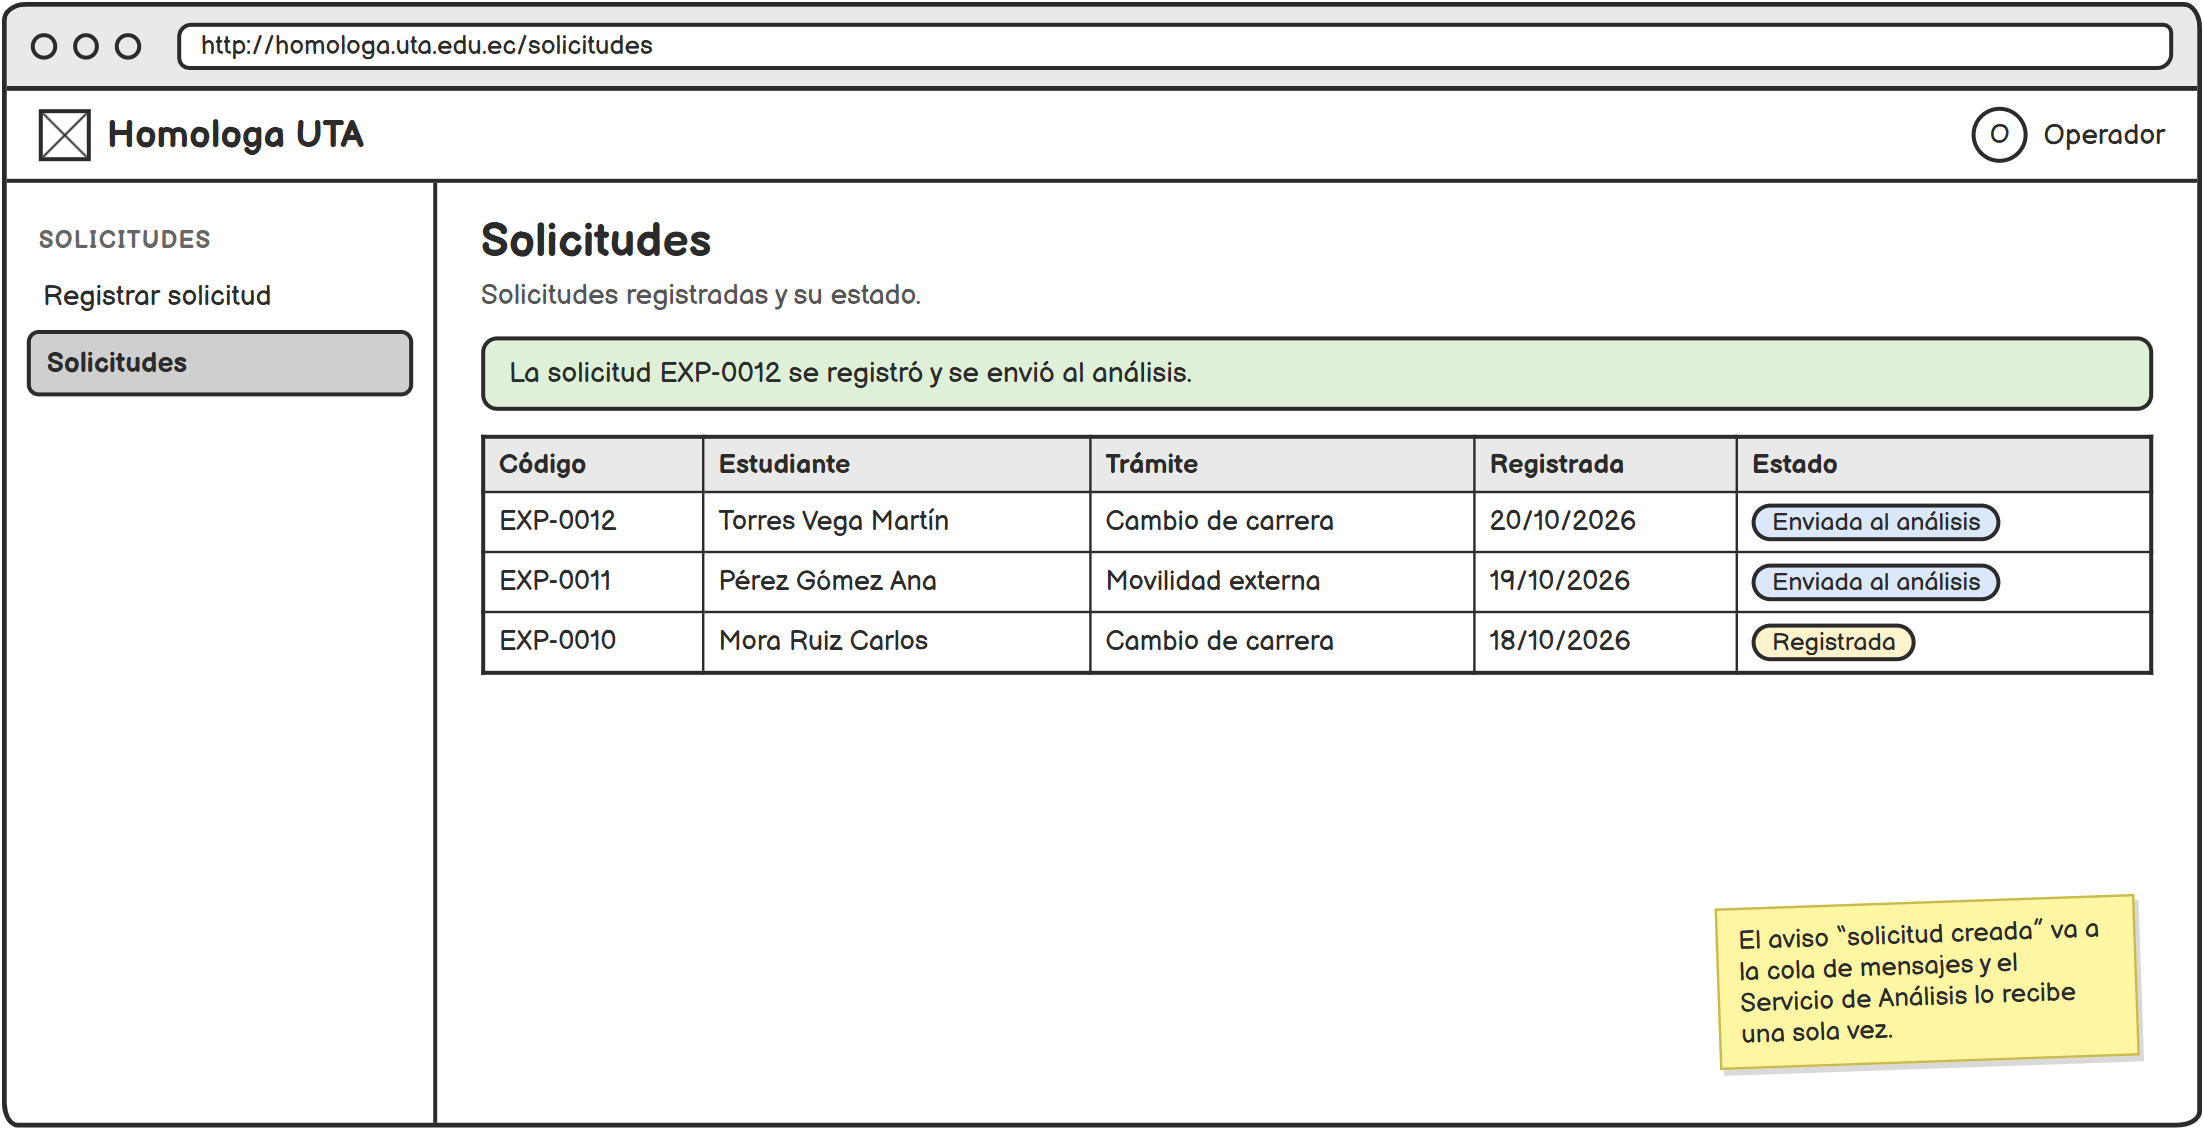
\includegraphics[width=0.93\textwidth]{mockups/m06.png}}
\caption{Mockup M-06 -- Solicitud enviada al análisis}
\end{figure}
\par\needspace{6\baselineskip}\noindent\textbf{\textit{Pruebas de aceptación -- HU-06}}\par
\begin{longtable}{|p{1.4cm}|p{3.7cm}|p{4.6cm}|p{5.1cm}|}
\hline\rowcolor{grisTarjeta}\textbf{N.º} & \textbf{Prueba} & \textbf{Entrada} & \textbf{Resultado esperado}\\\hline
\endhead
PA-06.1 & Publicación del evento en RabbitMQ & Después de registrar, se consultan las colas de RabbitMQ y el registro del Microservicio C. & Evento publicado y procesado\\\hline
\caption{Pruebas de aceptación de la HU-06}
\end{longtable}

\subsection{Incremento entregado y retrospectiva}
El informe del Sprint 2 señala como punto de partida que el Sprint 1 dejó usuarios y roles, reglas configurables, catálogo de carreras, entrada por Gateway y registro de solicitudes con sus PDF. La retrospectiva orientó mejoras en coordinación, integración y verificación continua; los hallazgos pendientes alimentaron el trabajo del Sprint 2.
